\documentclass[11pt]{article}
\usepackage[margin = 1in]{geometry}
\usepackage{amsmath}
\usepackage{amssymb}
\usepackage{amsthm}
\usepackage{graphicx}
\usepackage{enumitem}
\usepackage{url}
\usepackage[parfill]{parskip}
\usepackage{listings}
\newcommand{\skipline}{\vspace{\baselineskip}}
\newcommand{\spacer}{\noalign{\medskip}}
\newenvironment{problem}[1]{\textbf{Problem #1: }}{\newpage}
\usepackage{caption}
\usepackage{subcaption}
\usepackage[utf8]{inputenc}
\usepackage{xcolor}

\definecolor{codegreen}{rgb}{0,0.6,0}
\definecolor{codegray}{rgb}{0.5,0.5,0.5}
\definecolor{codepurple}{rgb}{0.58,0,0.82}
\definecolor{backcolour}{rgb}{0.95,0.95,0.92}

\lstdefinestyle{mystyle}{
	backgroundcolor=\color{backcolour},   
	commentstyle=\color{codegreen},
	keywordstyle=\color{magenta},
	numberstyle=\tiny\color{codegray},
	stringstyle=\color{codepurple},
	basicstyle=\ttfamily\footnotesize,
	breakatwhitespace=false,         
	breaklines=true,                 
	captionpos=b,                    
	keepspaces=true,                 
	numbers=left,                    
	numbersep=5pt,                  
	showspaces=false,                
	showstringspaces=false,
	showtabs=false,                  
	tabsize=2
}

\lstset{style=mystyle}
\begin{document}
	
	\begin{center}
		\textbf{Stephen Giang} \\
		\textbf{Computer Vision} \\
		\textbf{CS 559} \\
		\textbf{Stephen Giang RedID: 823184070} \\
		\skipline \skipline
	\end{center}

	\begin{problem}{1}
		Please answer the following questions precisely. Support your answer with equations, diagrams, etc, as appropriate.
		\begin{enumerate}[label = (\alph*)]
			\item Why is the assumption of image size as a power of 2 needed in Fast Fourier Transform (FFT)?
			\\ \\
			We assume that the image size is a power of 2 so that the recursive algorithm for FFT will have a time complexity of $\boldsymbol{O(n\log n )}$.  With every iteration of the algorithm, each component $F_e$ and $F_o$ can be broken down into its own components $F_{ee}, F_{eo}$ and $F_{oe}, F_{oo}$ respectively.
			\\
			\item What are the consequences of symmetricity and periodicity of the Fourier transform when displaying the Fourier spectrum? 
			\\ \\
			The consequences of symmetricity and periodicity of the Fourier Transform when displaying the Fourier Spectrum is that we can easily find the max values of the amplitude spectrum.  This also makes computations a lot more efficient as we know the entire amplitude spectrum from only a single period, as every period repeats. Lastly, the symmetricity and periodicity allows us to shift the Fourier Transform.
			\\
			\item Why is bit reversal needed for (FFT)?
			\\ \\
			Bit Reversal is needed in FFT to let the algorithm do its recursive nature of separability.  The bit reversal will be the algorithm that separates the arrays into its 2 sub arrays.  An example is the bit reversal will separate $f_e$ into $f_{ee}$ and $f_{eo}$ and vice versa.  
			\\
			\item What is the ringing effect and how is it reduced?
			\\ \\
			The ringing effect is something that happens to the Fourier transform due to sharp and sudden changes in the filter characteristics.  To reduce this effect, we can use two different smooth filers, the Butterworth or Gaussian low pass filters. 
			\\
			\item What are spectrum power and its relation to information contents of the image?
			\\ \\
			The power spectrum is related to the information contents of the image as:
			\[P(u,v) = |F(u,v)|^2 = R^2(u,v) + I^2(u,v)\]
			with the total power being:
			\[P_{total} = \sum_{u = 0}^{n - 1} \sum_{v = 0}^{n-1} P(u,v)\]
		\end{enumerate}	
	\end{problem}

	\begin{problem}{2}
		\begin{enumerate}[label = (\alph*)]
			\item Butterworth bandpass filter is described by $H_{bs} = \frac{1}{1+\left(\frac{w}{r^2 - r_0^2}\right)^{2p}}$ where $r = \sqrt{u^2 + v^2}$ and $w$ is the bandwidth and $r_0$ is the cutoff frequency. 
			\\ \\
			Propose the equation of a Guassian bandpass filter with a bandwidth $w$ and a cutoff frequency $r_0$.
			\\ \\
			Notice the following:
			\begin{align*}
				H_{lp} &= \frac{1}{1+\left(\frac{r}{r_0}\right)^{2p}}  & H_{bs} &= \frac{1}{1+\left(\frac{w}{r^2 - r_0^2}\right)^{2p}}  \\
				H_{hp} &= \frac{1}{1+\left(\frac{r_0}{r}\right)^{2p}} = 1 - \frac{1}{1+\left(\frac{r}{r_0}\right)^{2p}} &H_{bp} &= 1 - \frac{1}{1+\left(\frac{w}{r^2 - r_0^2}\right)^{2p}}  \\		
			\end{align*}
			So given $G_{lp}$ and $G_{hp}$, we can see the following:
			\begin{align*}
				G_{lp} &= e^{\frac{-1}{2}\left(\frac{r}{r_0}\right)^2} & \boldsymbol{G_{bs}} &= \boldsymbol{e^{\frac{-1}{2}\left(\frac{w}{r^2 - r_0^2}\right)^2}} \\
				G_{hp} &= 1 - e^{\frac{-1}{2}\left(\frac{r}{r_0}\right)^2} & \boldsymbol{G_{bp}} &= \boldsymbol{1 - e^{\frac{-1}{2}\left(\frac{w}{r^2 - r_0^2}\right)^2}}
			\end{align*}
			We can find the bandpass and bandstop filters by substituting $r / r_0$ with $w / (r^2 - r_0^2)$ 
			\\ \\
\begin{lstlisting}[language=Matlab]
brain = imread('../Figures/Brain.png');
r0 = 10;
wf = 10000;

[f0, f1, F1, Gbp, G, gflt, fflt] = GaussianBP(brain, r0, wf);

figure(), imshow( brain )
print -depsc ../Figures/Prob2/1.eps
figure(), imshow( uint8(f0) )
print -depsc ../Figures/Prob2/2.eps
figure(), imshow( uint8(f1) )
print -depsc ../Figures/Prob2/3.eps
figure(), imshow( mat2gray( log(abs(F1) + 1) ) )
print -depsc ../Figures/Prob2/4.eps
figure(), imshow( mat2gray( log(abs(Gbp) + 1) ) )
print -depsc ../Figures/Prob2/5.eps
figure(), imshow( mat2gray( log(abs(G) + 1) ) )
print -depsc ../Figures/Prob2/6.eps
figure(), imshow(uint8(gflt))
print -depsc ../Figures/Prob2/7.eps
figure(), imshow(uint8(fflt))
print -depsc ../Figures/Prob2/8.eps
\end{lstlisting}
			\newpage
\begin{lstlisting}[language=Matlab]
function [f0, f1, F1, Gbp, G, gflt, fflt] = GaussianBP(img, r0, wf)

% Padding for Size
w = size(img, 1);
h = size(img, 2);
power2 = 2 .^ (1 : 12);
for i = 1 : 12
	if max(w,h) <= power2(i)
		break
	end
end
n = power2(i);

f0 = zeros(n,n);
for i = 1 : w
	for j = 1 : h
		f0(i,j) = img(i,j);
	end
end

% Multiply by -1 ^ x+y
f1 = zeros(n,n);
for x = 1 : n
	for y = 1 : n
		f1(x,y) = (-1)^(x+y) * f0(x,y);
	end
end

% Fourier Transform
F1 = fft2(f1);

% Filter 
Gbp = zeros(n,n);
u = [(-n/2):((n/2) - 1), (-n/2):((n/2) - 1)];
[U,V] = meshgrid(u,u);
for i = 1 : n
	for j = 1 : n
		r2 = U(i,j)^2 + V(i,j)^2;
		frac = (-1/2) * ((wf)/(r2 - r0^2) )^2;
		Gbp(i,j) = 1 - exp(frac);
	end
end

% Multication of HF1
G = Gbp .* F1;

% Inverse
gflt = abs(ifft2(G));
fflt = gflt(1:w, 1:h);


end
\end{lstlisting}
			\newpage
			\item Demonstrate the usefulness of the Gaussian bandpass filter using an image of your choice.  Discuss the results. 
			\begin{figure}[h!]
				\centering
				\begin{subfigure}[h!]{.3\textwidth}
					\centering
					\includegraphics[height = 4cm]{Figures/Prob2/1}
					\caption{Original image}
				\end{subfigure}
				\begin{subfigure}[h!]{.3\textwidth}
					\centering
					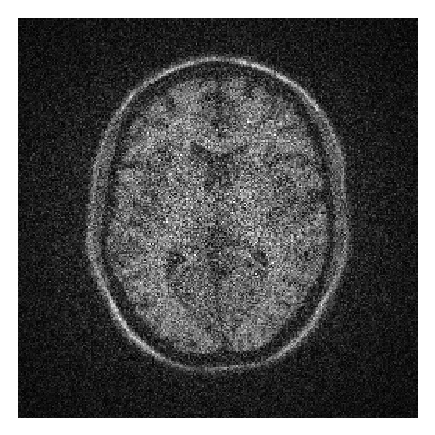
\includegraphics[height = 4cm]{Figures/Prob2/2}
					\caption{Resized image $f_0$}
				\end{subfigure}
				\begin{subfigure}[h!]{.3\textwidth}
					\centering
					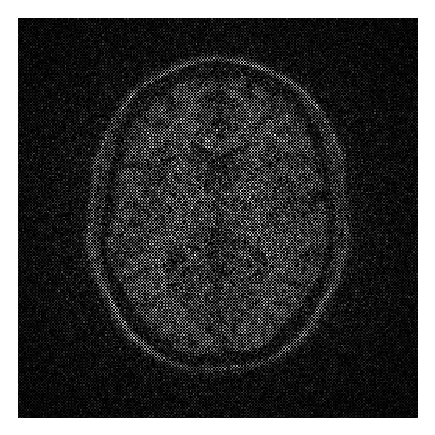
\includegraphics[height = 4cm]{Figures/Prob2/3}
					\caption{$f_1 = -1^{x+y}f_0$}
				\end{subfigure}
			\end{figure}
			\begin{figure}[h!]
				\centering
				\begin{subfigure}[h!]{.3\textwidth}
					\centering
					\includegraphics[height = 4cm]{Figures/Prob2/4}
					\caption{Fourier Transform of $f_1$, $F_1$}
				\end{subfigure}
				\begin{subfigure}[h!]{.3\textwidth}
					\centering
					
\includegraphics[height = 4cm]{Figures/Prob2/5}
					\caption{Gaussian LP $G_{lp}$}
				\end{subfigure}
				\begin{subfigure}[h!]{.3\textwidth}
					\centering
					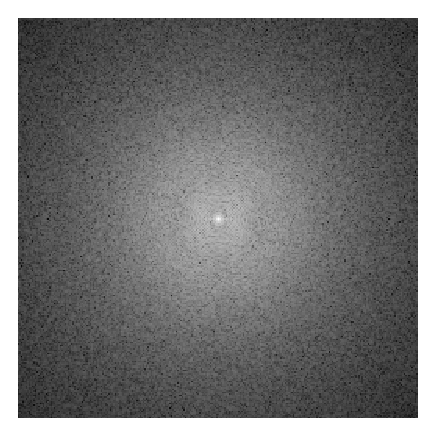
\includegraphics[height = 4cm]{Figures/Prob2/6}
					\caption{$G = G_{bp}F_1$}
				\end{subfigure}
			\end{figure}
			\begin{figure}[h!]
				\centering
				\begin{subfigure}[h!]{.4\textwidth}
					\centering
					\includegraphics[height = 4cm]{Figures/Prob2/7}
					\caption{Inverse Fourier Transform of G, $g_{flt}$}
				\end{subfigure}
				\begin{subfigure}[h!]{.4\textwidth}
					\centering
					\includegraphics[height = 4cm]{Figures/Prob2/8}
					\caption{Resized to Original $f_{flt}$}
				\end{subfigure}
			\end{figure}
			\\ \\
			The usefulness of the Gaussian Bandpass filter is that we are able to make a more specified frequency domain.  The low pass filters remove the high frequency components and the high pass removes the lower frequencies.  With the bandpass, we are able to set bounds and specify which frequencies to keep and which to remove.  It can be very useful when one needs specified frequencies in medical technologies such as brain scans.  
		\end{enumerate}
	\end{problem}

	\begin{problem}{3}
		Consider Lena.png image below
		\begin{figure}[h!]
			\centering
			\includegraphics[height = 6cm]{Figures/Lena.png}
		\end{figure}
		\begin{enumerate}[label = (\alph*)]
			\item Propose and apply a suitable filter (in the frequency or spatial domain) to remove the lines from the image and clean it as much as possible.
			\\ \\
			Notice that the lines on the image represents sinusoidal noise.  For this, we can apply the \textbf{Butterworth Low Pass Filter.}
			\\ \\
\begin{lstlisting}[language=Matlab]
lena = rgb2gray(imread('../Figures/Lena.png'));

[f0, f1, F1, Hlp, G, gflt, fflt] = ButterworthLP(lena, 45, 6);

figure(), imshow( lena )
print -depsc ../Figures/Prob3/1.eps

figure(), imshow( uint8(f0) )
print -depsc ../Figures/Prob3/2.eps

figure(), imshow( uint8(f1) )
print -depsc ../Figures/Prob3/3.eps

figure(), imshow( mat2gray( log(abs(F1) + 1) ) )
print -depsc ../Figures/Prob3/4.eps

figure(), imshow( mat2gray( log(abs(Hlp) + 1) ) )
print -depsc ../Figures/Prob3/5.eps

figure(), imshow( mat2gray( log(abs(G) + 1) ) )
print -depsc ../Figures/Prob3/6.eps

figure(), imshow(uint8(gflt))
print -depsc ../Figures/Prob3/7.eps

figure(), imshow(uint8(abs(fflt)))
print -depsc ../Figures/Prob3/8.eps
\end{lstlisting}
			\newpage
\begin{lstlisting}[language=Matlab]
function [f0, f1, F1, Hlp, G, gflt, fflt] = ButterworthLP(img, r0, p)

	% Padding for Size
	w = size(img, 1);
	h = size(img, 2);
	power2 = 2 .^ (1 : 12);
	for i = 1 : 12
		if max(w,h) <= power2(i)
			break
		end
	end
	n = power2(i);
	
	f0 = zeros(n,n);
	for i = 1 : w
		for j = 1 : h
			f0(i,j) = img(i,j);
		end
	end
	
	% Multiply by -1 ^ x+y
	f1 = zeros(n,n);
	for x = 1 : n
		for y = 1 : n
			f1(x,y) = (-1)^(x+y) * f0(x,y);
		end
	end
	
	% Fourier Transform
	F1 = fft2(f1);
	
	% Filter 
	Hlp = zeros(n,n);
	u = [(-n/2):((n/2) - 1), (-n/2):((n/2) - 1)];
	[U,V] = meshgrid(u,u);
	for i = 1 : n
		for j = 1 : n
			r = sqrt(U(i,j)^2 + V(i,j)^2);
			frac = (r / r0)^(2*p);
			Hlp(i,j) = 1 / (1 + frac);
		end
	end
	
	% Multication of HF1
	G = Hlp .* F1;
	
	% Inverse
	gflt = abs(ifft2(G));
	fflt = gflt(1:w, 1:h);

end
\end{lstlisting}
			\newpage
			\item Provide all images, e.g. Fourier spectrum (if applicable), etc. and clearly label figures with suitable captions.
			\begin{figure}[h!]
				\centering
				\begin{subfigure}[h!]{.3\textwidth}
					\centering
					\includegraphics[height = 4cm]{Figures/Prob3/1}
					\caption{Original image}
				\end{subfigure}
				\begin{subfigure}[h!]{.3\textwidth}
					\centering
					\includegraphics[height = 4cm]{Figures/Prob3/2}
					\caption{Resized image $f_0$}
				\end{subfigure}
				\begin{subfigure}[h!]{.3\textwidth}
					\centering
					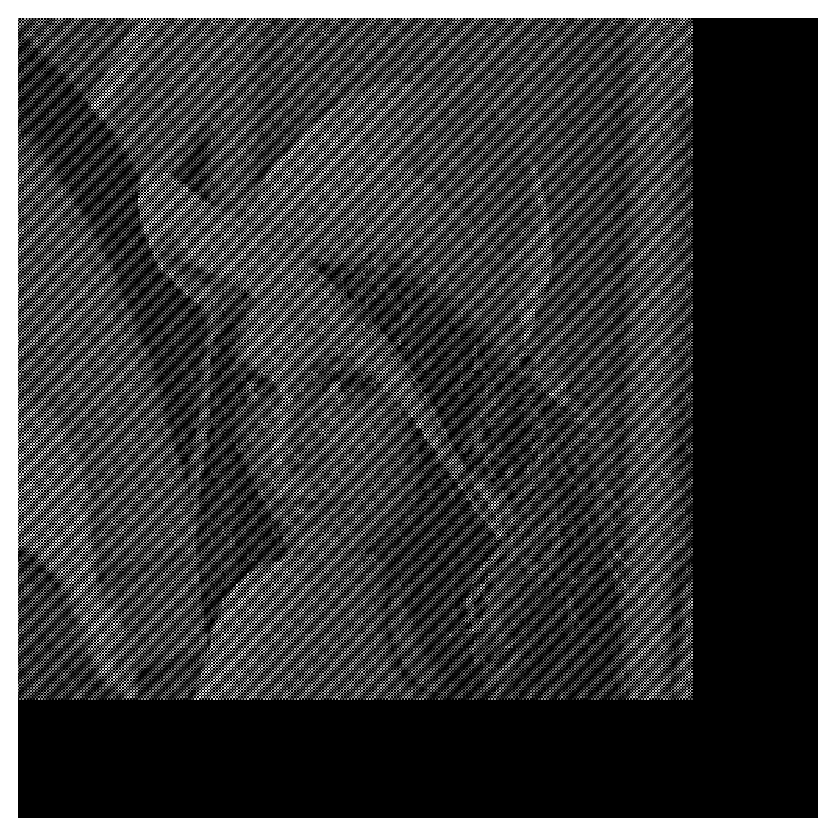
\includegraphics[height = 4cm]{Figures/Prob3/3}
					\caption{$f_1 = -1^{x+y}f_0$}
				\end{subfigure}
			\end{figure}
			\begin{figure}[h!]
				\centering
				\begin{subfigure}[h!]{.3\textwidth}
					\centering
					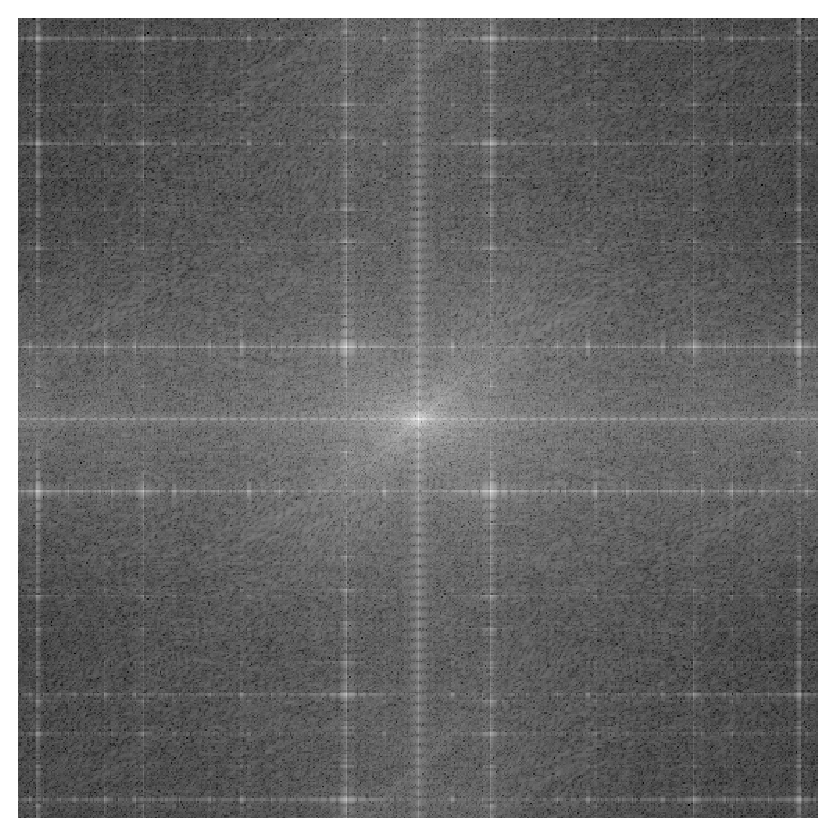
\includegraphics[height = 4cm]{Figures/Prob3/4}
					\caption{Fourier Transform of $f_1$, $F_1$}
				\end{subfigure}
				\begin{subfigure}[h!]{.3\textwidth}
					\centering
					
\includegraphics[height = 4cm]{Figures/Prob3/5}
					\caption{Butterworth LP $H_{lp}$}
				\end{subfigure}
				\begin{subfigure}[h!]{.3\textwidth}
					\centering
					\includegraphics[height = 4cm]{Figures/Prob3/6}
					\caption{$G = H_{lp}F_1$}
				\end{subfigure}
			\end{figure}
			\begin{figure}[h!]
				\centering
				\begin{subfigure}[h!]{.4\textwidth}
					\centering
					\includegraphics[height = 4cm]{Figures/Prob3/7}
					\caption{Inverse Fourier Transform of G, $g_{flt}$}
				\end{subfigure}
				\begin{subfigure}[h!]{.4\textwidth}
					\centering
					\includegraphics[height = 4cm]{Figures/Prob3/8}
					\caption{Resized to Original $f_{flt}$}
				\end{subfigure}
			\end{figure}
			\newpage
			\item Discuss the reason for the choice (including filter parameters such as cutoff frequency, etc.) and effectiveness of your filter, and the possible challenges in reduction of the type of noise in the above image.
			\\ \\
			I decided to a Butterworth Low Pass filter on this image because the image originally contained sinusoidal noise.  With sinusoidal noise, the Butterworth will remove the high frequencies, whereas the median and mean filters would simply average the noise and the signal.  With Butterworth, it removes the distinct parts of the image, such as the noise, and produces a more smooth, but blurry image. I noticed that as $r_0$ increases, it looks more and more like the original image.  As $r_0$ decreases, the image becomes more smooth and more blurry. As a nice median, I chose $r_0 = 45$.  As $p$ increase, we see that the final result contains less and less noise. However, I did notice that for $p > 6$, we get that the final result has horizontal lines for noise.  So thats why I chose, $p = 6$. With the following parameters, I think I got a very nice image and the filter was very effective.  The only challenges would be finding the right parameters. 
			\newpage
			Notice the following images with varied $r_0$ values with a constant $p = 6$:
			\\
			\begin{figure}[h!]
				\centering
				\begin{subfigure}{.3 \textwidth}
					\centering
					
\includegraphics[height = 3.5cm]{Figures/Prob3/r01}
					\caption{$r_0 = 1$}
				\end{subfigure}
				\begin{subfigure}{.3 \textwidth}
					\centering
					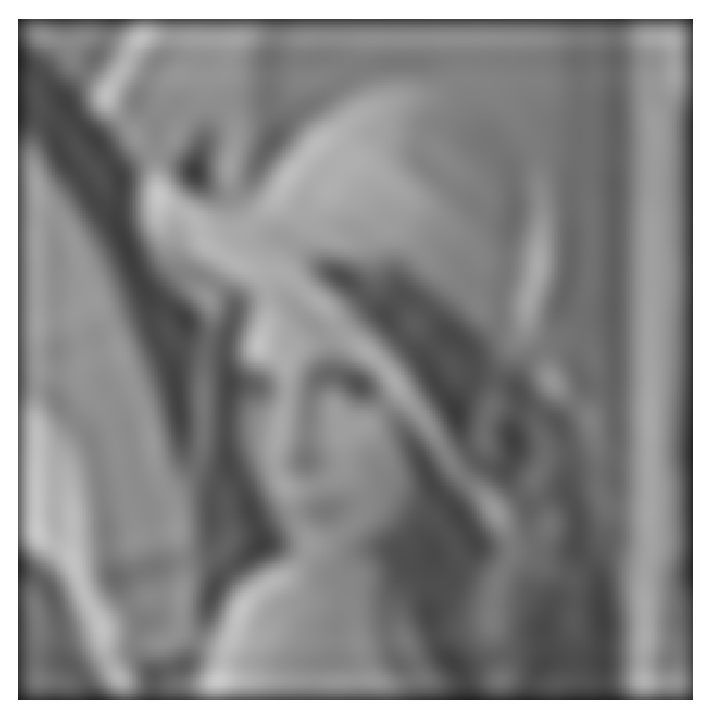
\includegraphics[height = 3.5cm]{Figures/Prob3/r020}
					\caption{$r_0 = 20$}
				\end{subfigure}
				\begin{subfigure}{.3 \textwidth}
					\centering
					\includegraphics[height = 3.5cm]{Figures/Prob3/r040}
					\caption{$r_0 = 40$}
				\end{subfigure}
			\end{figure}
			\begin{figure}[h!]
				\centering
				\begin{subfigure}{.3 \textwidth}
					\centering
					\includegraphics[height = 3.5cm]{Figures/Prob3/r060}
					\caption{$r_0 = 60$}
				\end{subfigure}
				\begin{subfigure}{.3 \textwidth}
					\centering
					\includegraphics[height = 3.5cm]{Figures/Prob3/r080}
					\caption{$r_0 = 80$}
				\end{subfigure}
				\begin{subfigure}{.3 \textwidth}
					\centering
					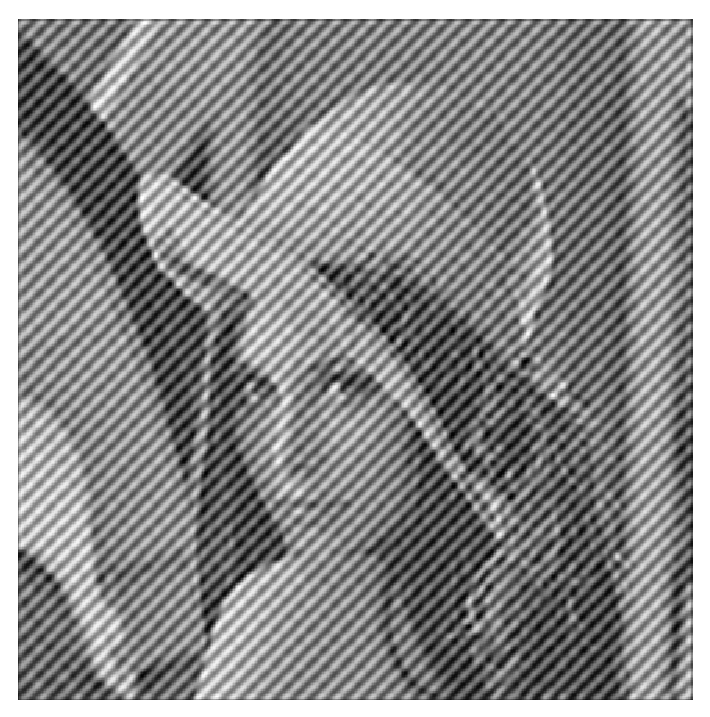
\includegraphics[height = 3.5cm]{Figures/Prob3/r0100}
					\caption{$r_0 = 100$}
				\end{subfigure}
			\end{figure}
			\\ 
			Notice the following images with varied $p$ values with a constant $r_0 = 45$:
			\\
			\begin{figure}[h!]
				\centering
				\begin{subfigure}{.3 \textwidth}
					\centering
					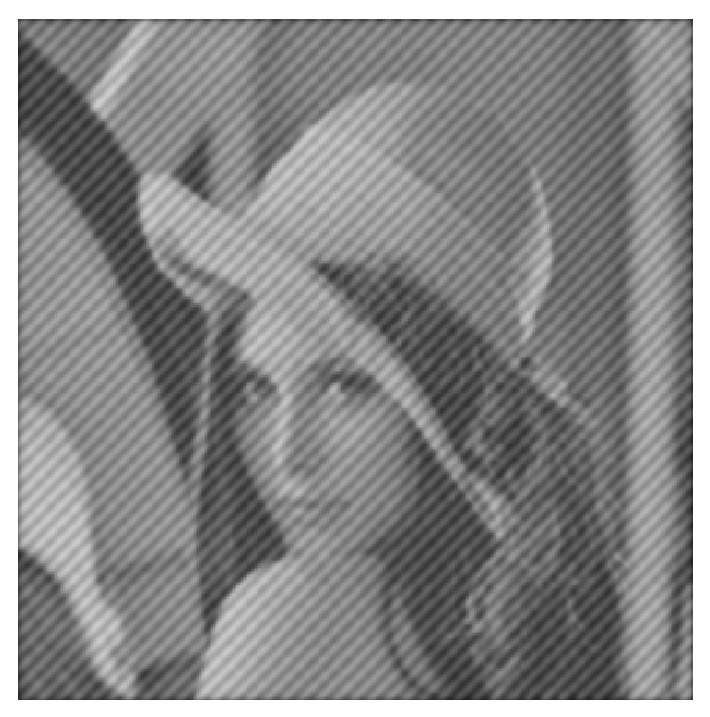
\includegraphics[height = 3.5cm]{Figures/Prob3/p1}
					\caption{$r_0 = 1$}
				\end{subfigure}
				\begin{subfigure}{.3 \textwidth}
					\centering
					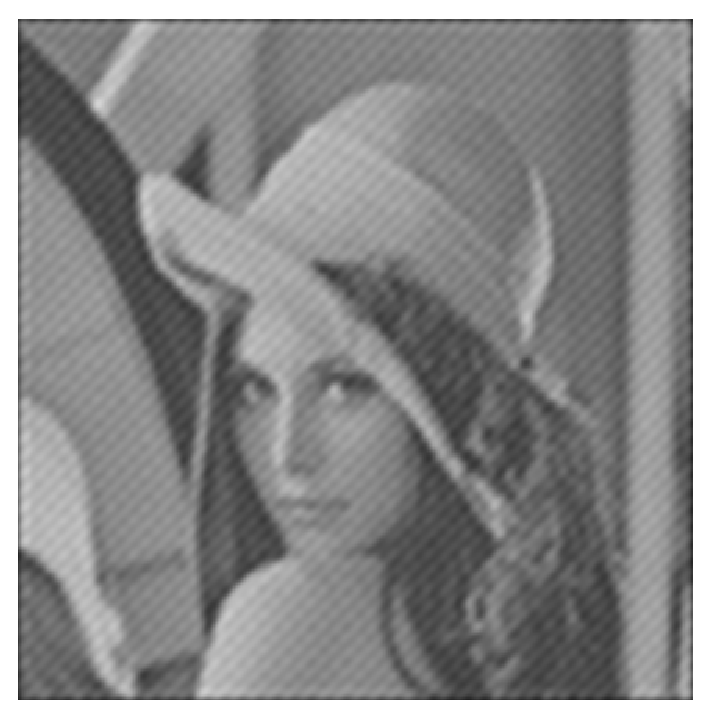
\includegraphics[height = 3.5cm]{Figures/Prob3/p3}
					\caption{$r_0 = 20$}
				\end{subfigure}
				\begin{subfigure}{.3 \textwidth}
					\centering
					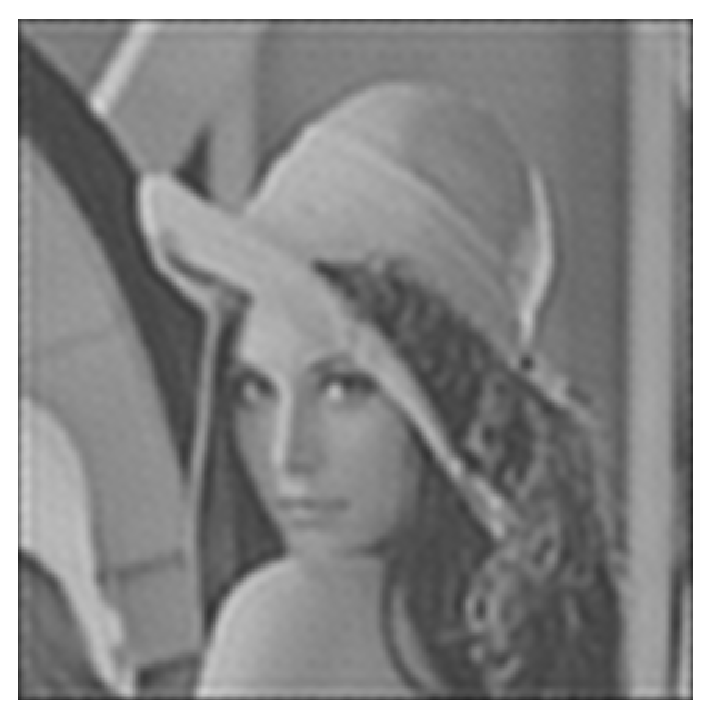
\includegraphics[height = 3.5cm]{Figures/Prob3/p6}
					\caption{$r_0 = 40$}
				\end{subfigure}
			\end{figure}
			\begin{figure}[h!]
				\centering
				\begin{subfigure}{.3 \textwidth}
					\centering
					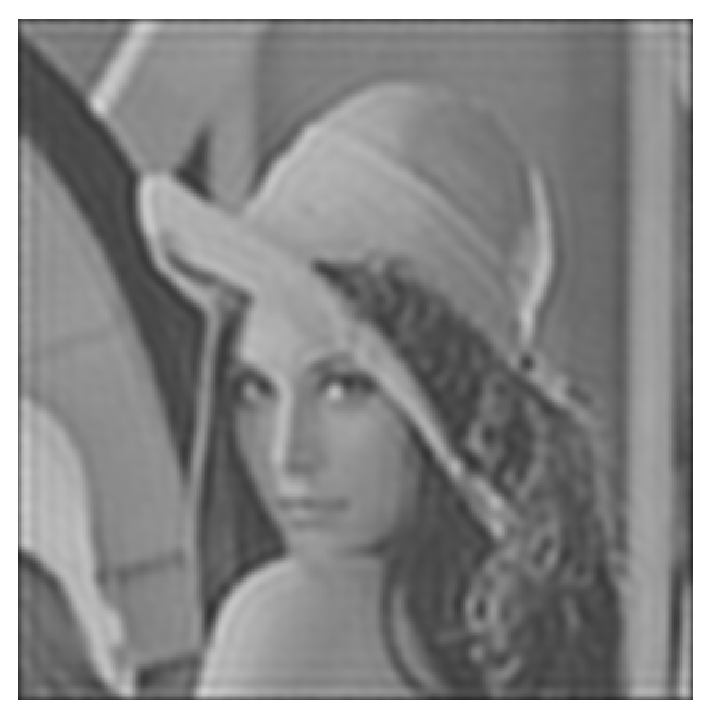
\includegraphics[height = 4cm]{Figures/Prob3/p10}
					\caption{$r_0 = 60$}
				\end{subfigure}
				\begin{subfigure}{.3 \textwidth}
					\centering
					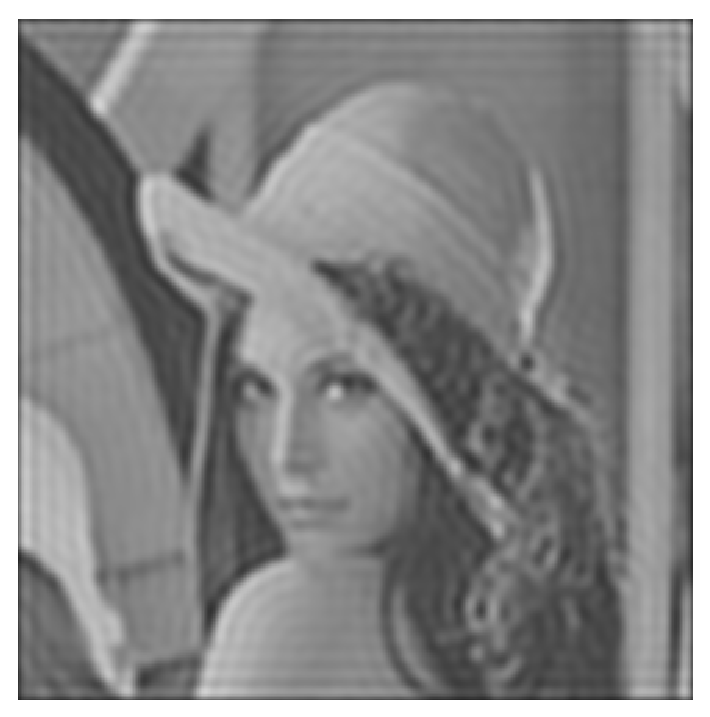
\includegraphics[height = 4cm]{Figures/Prob3/p25}
					\caption{$r_0 = 80$}
				\end{subfigure}
				\begin{subfigure}{.3 \textwidth}
					\centering
					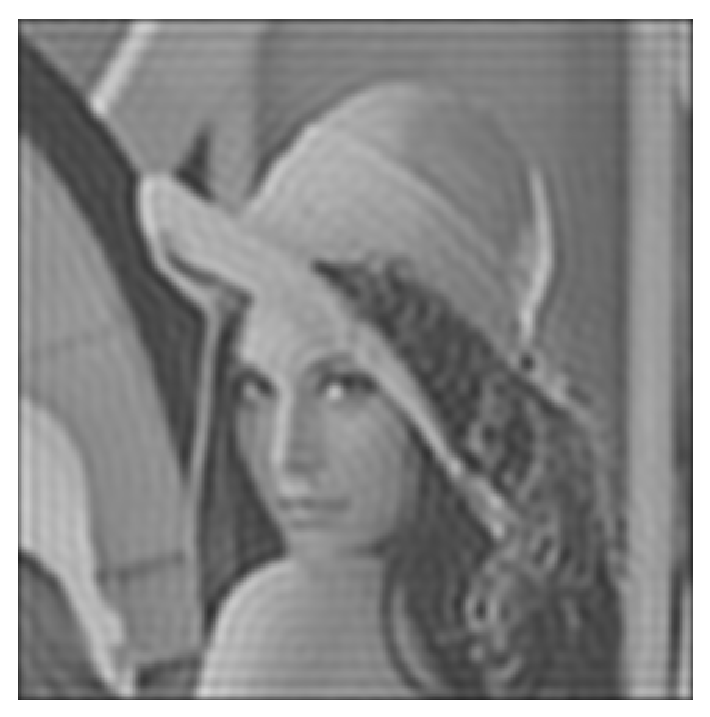
\includegraphics[height = 4cm]{Figures/Prob3/p100}
					\caption{$r_0 = 100$}
				\end{subfigure}
			\end{figure}
		\end{enumerate}
	\end{problem}

	\begin{problem}{4}
		Consider the image shown below
		\begin{figure}[h!]
			\centering
			\includegraphics[height = 6cm]{Figures/Lena2.png}
		\end{figure}
		\begin{enumerate}[label = (\alph*)]
			\item Propose and apply a suitable filter (in the frequency or spatial domain) to remove the lines from the image and clean it as much as possible.
			\\ \\
			Notice how the static looks like Gaussian noise, so we can apply a \textbf{Gaussian Low Pass Filter.}
			\\ \\
\begin{lstlisting}[language=Matlab]
lena2 = rgb2gray(imread('../Figures/Lena2.png'));

[f0, f1, F1, Glp, G, gflt, fflt] = GaussianLP(lena2, 40);


figure(), imshow( lena2 )
print -depsc ../Figures/Prob4/1.eps

figure(), imshow( uint8(f0) )
print -depsc ../Figures/Prob4/2.eps

figure(), imshow( uint8(f1) )
print -depsc ../Figures/Prob4/3.eps

figure(), imshow( mat2gray( log(abs(F1) + 1) ) )
print -depsc ../Figures/Prob4/4.eps

figure(), imshow( mat2gray( log(abs(Glp) + 1) ) )
print -depsc ../Figures/Prob4/5.eps

figure(), imshow( mat2gray( log(abs(G) + 1) ) )
print -depsc ../Figures/Prob4/6.eps

figure(), imshow(uint8(gflt))
print -depsc ../Figures/Prob4/7.eps

figure(), imshow(uint8(fflt))
print -depsc ../Figures/Prob4/8.eps
\end{lstlisting}
			\newpage
\begin{lstlisting}[language=Matlab]
function [f0, f1, F1, Glp, G, gflt, fflt] = GaussianLP(img, r0)

% Padding for Size
w = size(img, 1);
h = size(img, 2);
power2 = 2 .^ (1 : 12);
for i = 1 : 12
	if max(w,h) <= power2(i)
		break
	end
end
n = power2(i);

f0 = zeros(n,n);
for i = 1 : w
	for j = 1 : h
		f0(i,j) = img(i,j);
	end
end

% Multiply by -1 ^ x+y
f1 = zeros(n,n);
for x = 1 : n
	for y = 1 : n
		f1(x,y) = (-1)^(x+y) * f0(x,y);
	end
end

% Fourier Transform
F1 = fft2(f1);

% Filter 
Glp = zeros(n,n);
u = [(-n/2):((n/2) - 1), (-n/2):((n/2) - 1)];
[U,V] = meshgrid(u,u);
for i = 1 : n
	for j = 1 : n
		r2 = U(i,j)^2 + V(i,j)^2;
		frac = (-r2) / (2 * (r0)^2);
		Glp(i,j) = exp(frac);
	end
end

% Multication of HF1
G = Glp .* F1;

% Inverse
gflt = abs(ifft2(G));
fflt = gflt(1:w, 1:h);

end
\end{lstlisting}
			\newpage
			\item Provide all images, e.g. Fourier spectrum (if applicable), etc. and clearly label figures with suitable captions.
			\begin{figure}[h!]
				\centering
				\begin{subfigure}[h!]{.3\textwidth}
					\centering
					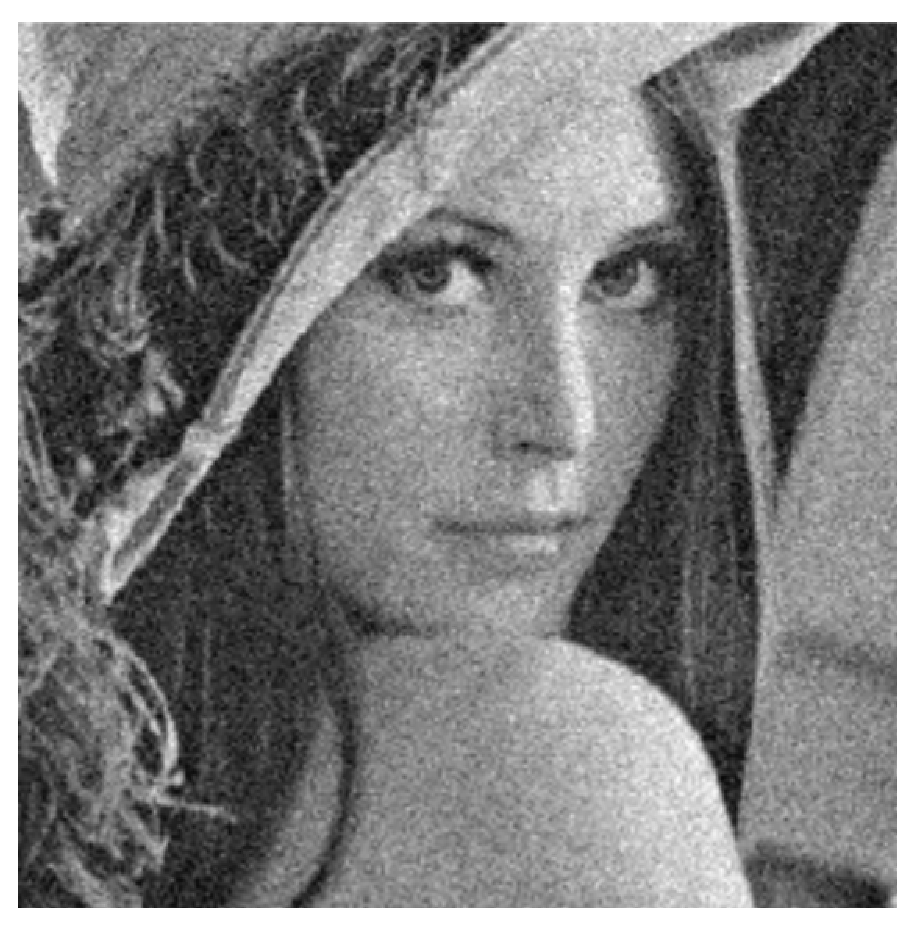
\includegraphics[height = 4cm]{Figures/Prob4/1}
					\caption{Original image}
				\end{subfigure}
				\begin{subfigure}[h!]{.3\textwidth}
					\centering
					\includegraphics[height = 4cm]{Figures/Prob4/2}
					\caption{Resized image $f_0$}
				\end{subfigure}
				\begin{subfigure}[h!]{.3\textwidth}
					\centering
					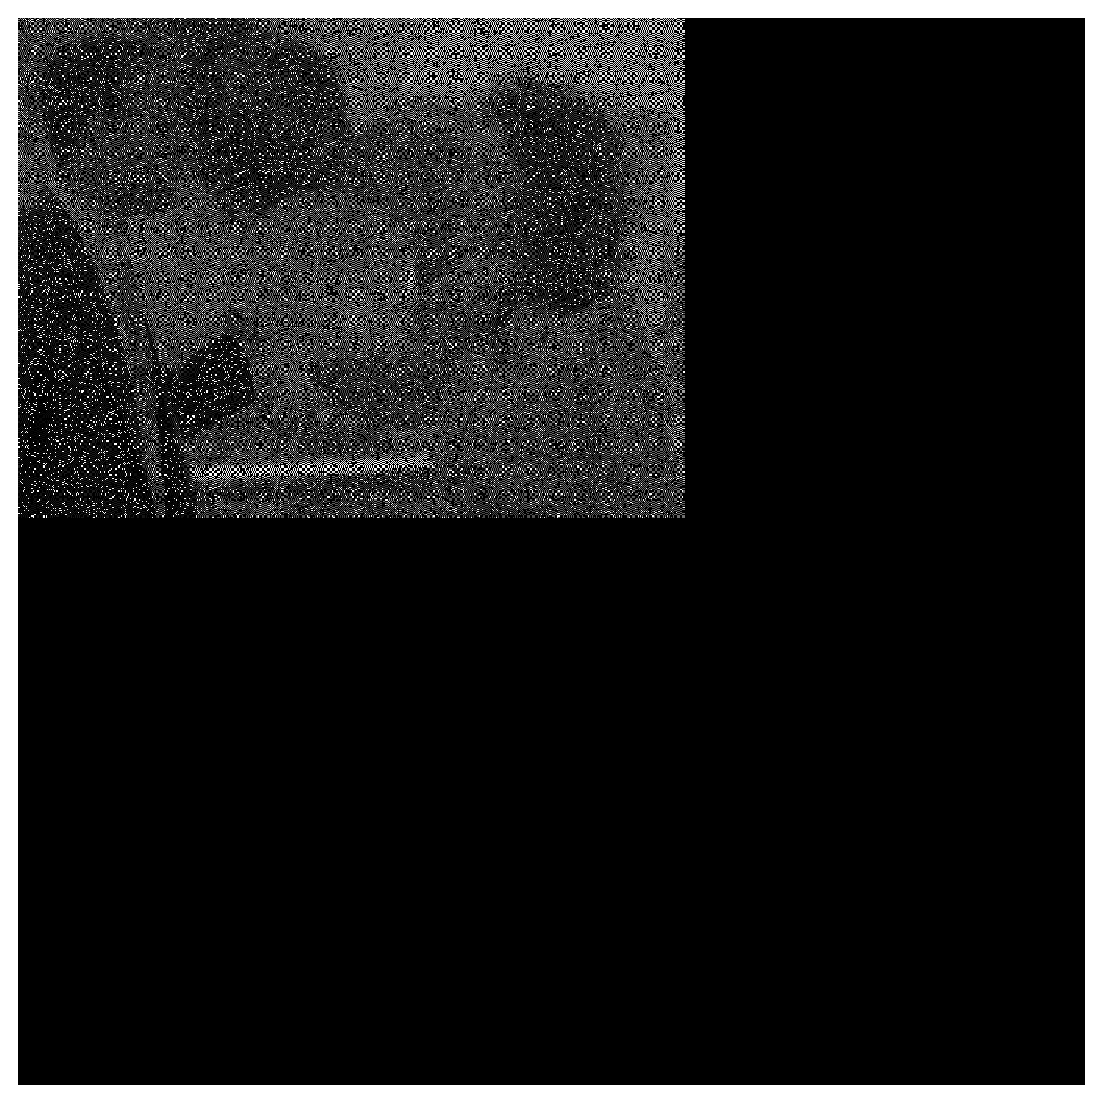
\includegraphics[height = 4cm]{Figures/Prob4/3}
					\caption{$f_1 = -1^{x+y}f_0$}
				\end{subfigure}
			\end{figure}
			\begin{figure}[h!]
				\centering
				\begin{subfigure}[h!]{.3\textwidth}
					\centering
					\includegraphics[height = 4cm]{Figures/Prob4/4}
					\caption{Fourier Transform of $f_1$, $F_1$}
				\end{subfigure}
				\begin{subfigure}[h!]{.3\textwidth}
					\centering
					
\includegraphics[height = 4cm]{Figures/Prob4/5}
					\caption{Gaussian LP $G_{lp}$}
				\end{subfigure}
				\begin{subfigure}[h!]{.3\textwidth}
					\centering
					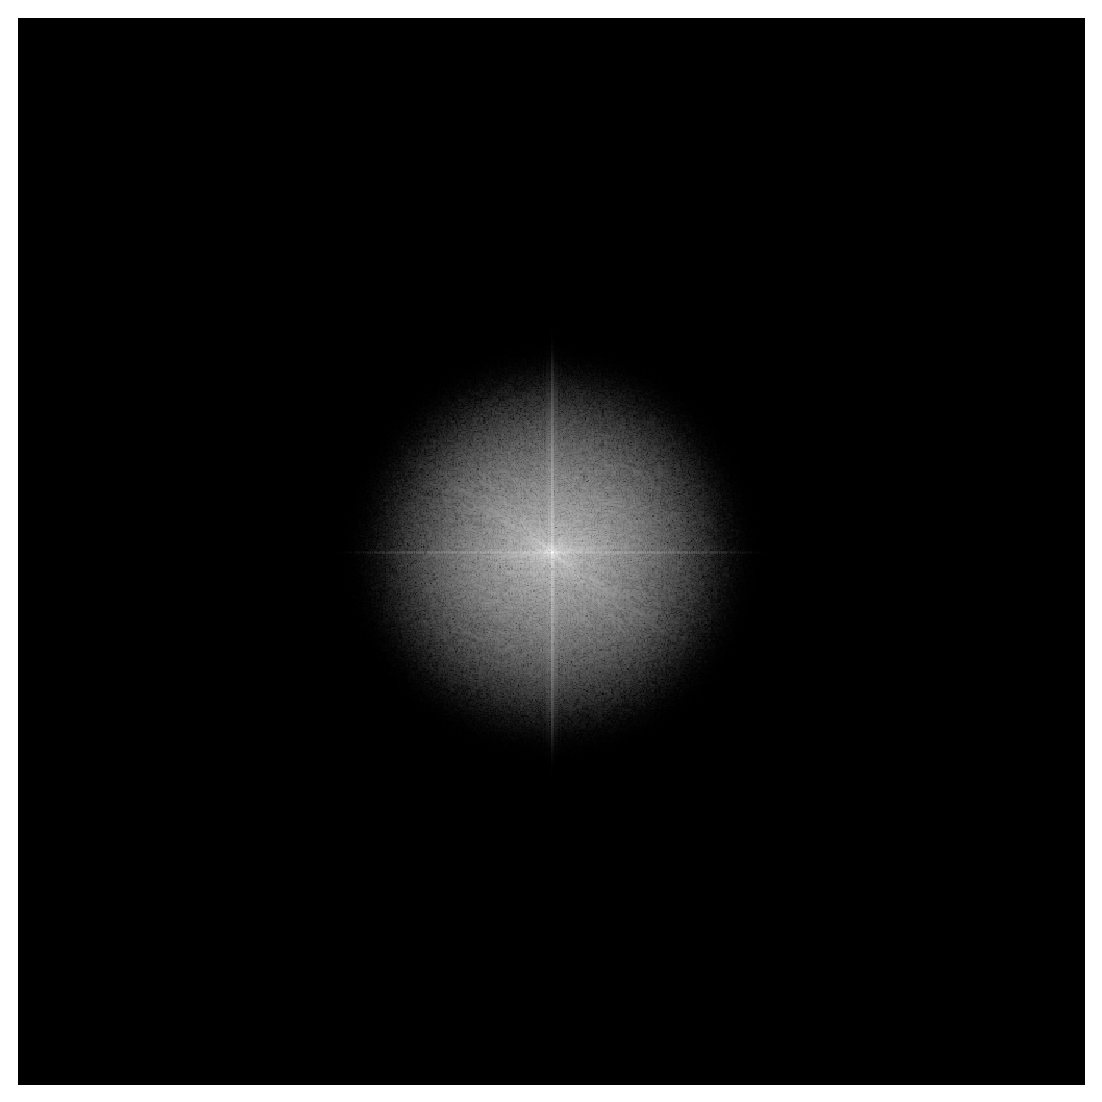
\includegraphics[height = 4cm]{Figures/Prob4/6}
					\caption{$G = G_{lp}F_1$}
				\end{subfigure}
			\end{figure}
			\begin{figure}[h!]
				\centering
				\begin{subfigure}[h!]{.4\textwidth}
					\centering
					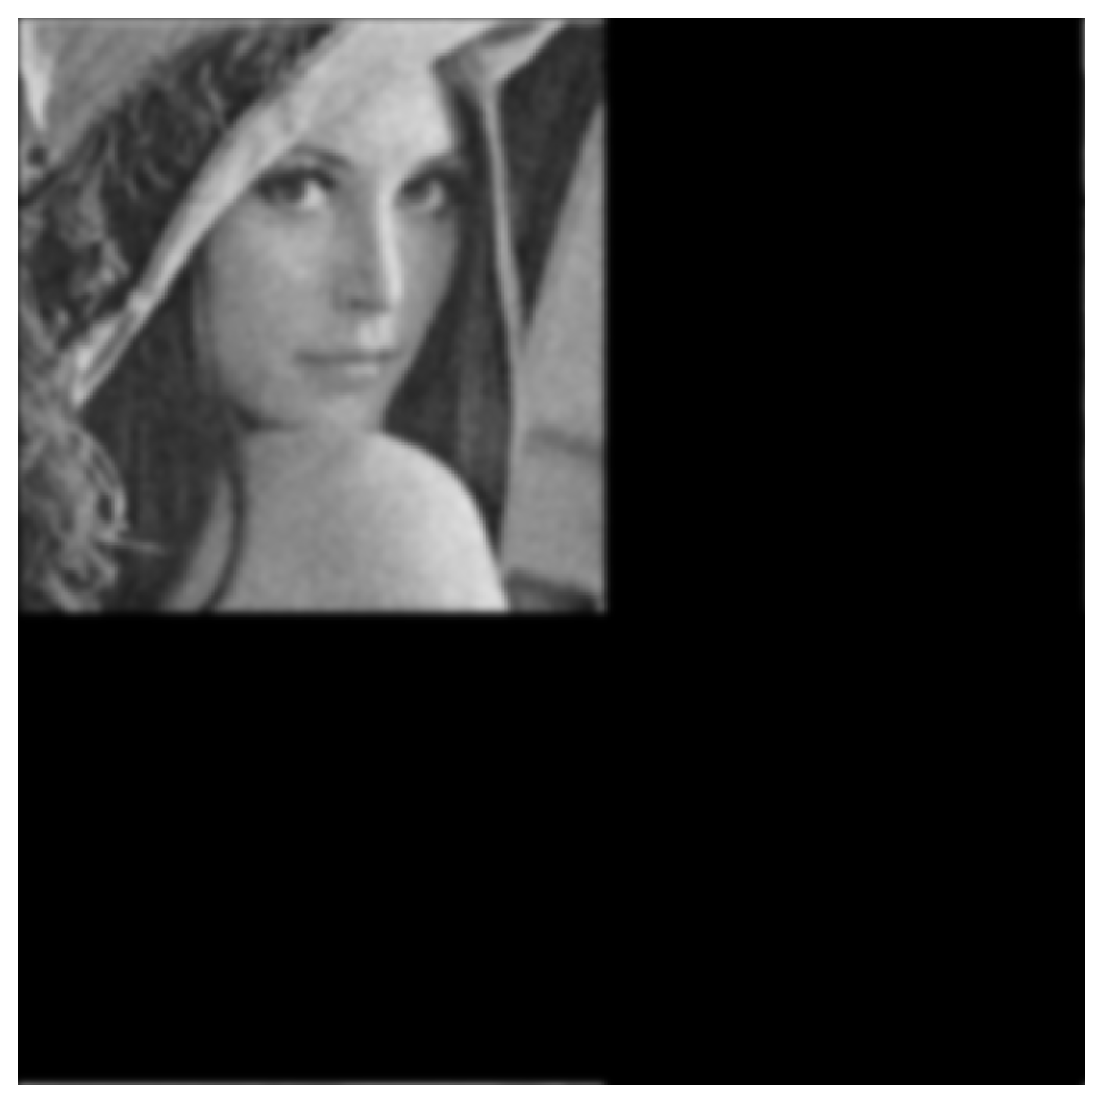
\includegraphics[height = 4cm]{Figures/Prob4/7}
					\caption{Inverse Fourier Transform of G, $g_{flt}$}
				\end{subfigure}
				\begin{subfigure}[h!]{.4\textwidth}
					\centering
					\includegraphics[height = 4cm]{Figures/Prob4/8}
					\caption{Resized to Original $f_{flt}$}
				\end{subfigure}
			\end{figure}
			\newpage
			\item Discuss the reason for the choice (including filter parameters such as cutoff frequency, etc.) and effectiveness of your filter, and the possible challenges in reduction of the type of noise in the above image.
			\\ \\
			For this image, I saw that it contains a lot of Gaussian noise, so I decided to use the Gaussian Low Pass Filter.  I noticed that for small $r_0$, the image would be very smooth/blurry, and for large $r_0$, the image did not remove enough noise.  So I had to choose a not too small, and not too large $r_0 = 40$ to get the desired result.  For the effectiveness of the filter, I would say it produced an okay image.  We can still see some noise, but if I were to remove more noise, the picture would be too smooth/blurry.  The challenge here is simply finding a perfect parameter value. 
			\\ \\
			Notice the following images with varied $r_0$ values:
			\\
			\begin{figure}[h!]
				\centering
				\begin{subfigure}{.3 \textwidth}
					\centering
					
\includegraphics[height = 4cm]{Figures/Prob4/r01}
					\caption{$r_0 = 1$}
				\end{subfigure}
				\begin{subfigure}{.3 \textwidth}
					\centering
					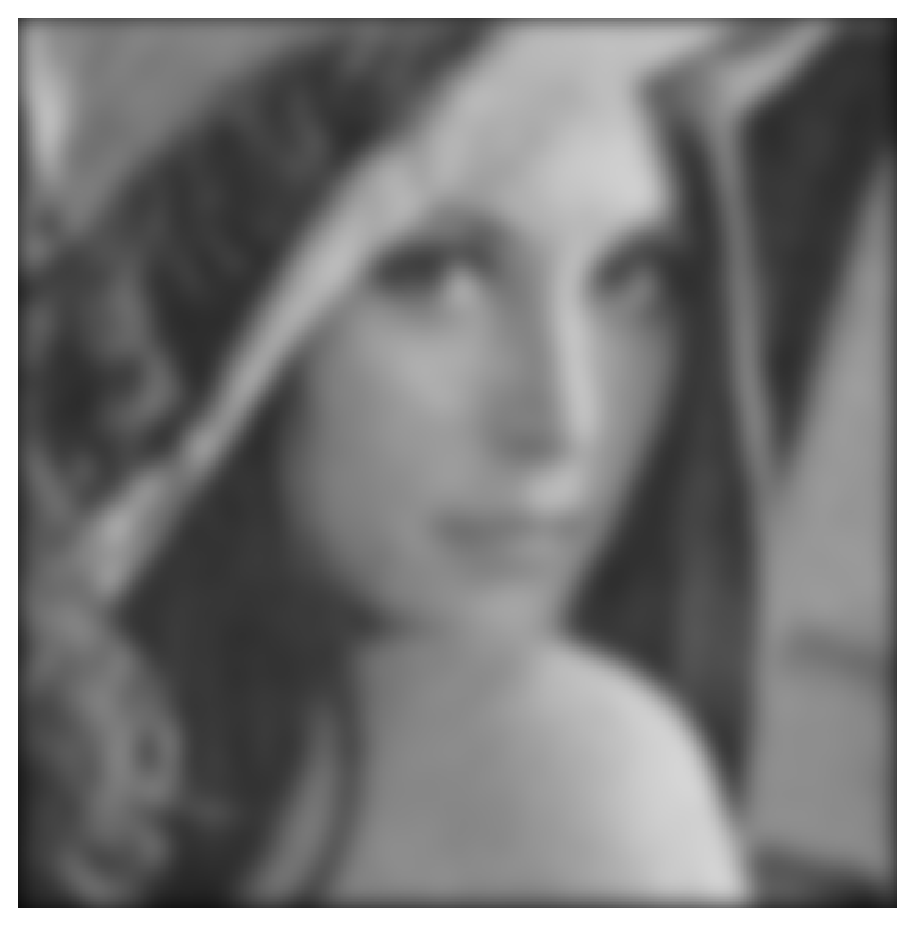
\includegraphics[height = 4cm]{Figures/Prob4/r020}
					\caption{$r_0 = 20$}
				\end{subfigure}
				\begin{subfigure}{.3 \textwidth}
					\centering
					\includegraphics[height = 4cm]{Figures/Prob4/r040}
					\caption{$r_0 = 40$}
				\end{subfigure}
			\end{figure}
			\begin{figure}[h!]
				\centering
				\begin{subfigure}{.3 \textwidth}
					\centering
					\includegraphics[height = 4cm]{Figures/Prob4/r060}
					\caption{$r_0 = 60$}
				\end{subfigure}
				\begin{subfigure}{.3 \textwidth}
					\centering
					\includegraphics[height = 4cm]{Figures/Prob4/r080}
					\caption{$r_0 = 80$}
				\end{subfigure}
				\begin{subfigure}{.3 \textwidth}
					\centering
					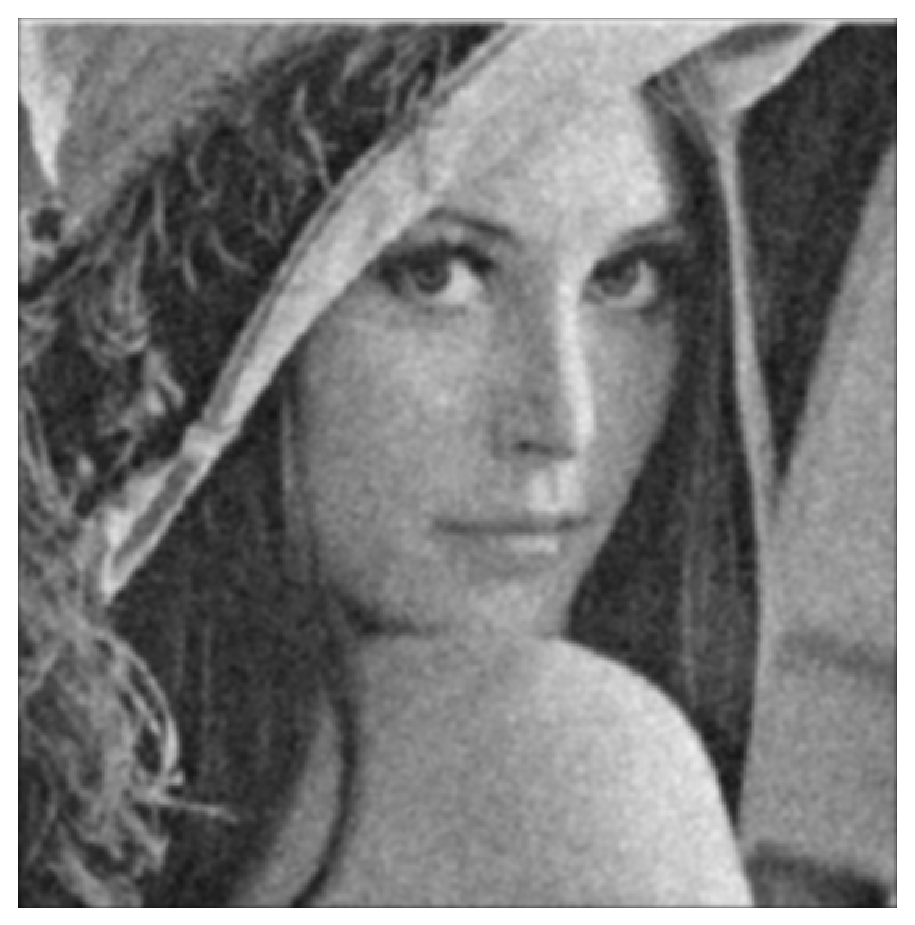
\includegraphics[height = 4cm]{Figures/Prob4/r0100}
					\caption{$r_0 = 100$}
				\end{subfigure}
			\end{figure}
		\end{enumerate}
	\end{problem}

	\begin{problem}{5}
		Consider the image shown below
		\begin{figure}[h!]
			\centering
			\includegraphics[height = 6cm]{Figures/Balloons.png}
		\end{figure}
		\begin{enumerate}[label = (\alph*)]
			\item Propose and apply a suitable filter (in the frequency or spatial domain) to remove the lines from the image and clean it as much as possible.
			\\ \\
			Because of all the salt and pepper noise, we can use the \textbf{Gaussian Low Pass Filter on each of the RGB components of the colored image.}
			\\ \\
\begin{lstlisting}[language=Matlab]
balloons = imread('../Figures/balloons.png');

figure(), imshow( balloons )

red = balloons(:,:,1);
green = balloons(:,:,2);
blue = balloons(:,:,3);

r0 = 30;

[f0, f1, F1, Glp, G, gflt, fflt1] = GaussianLP(red, r0);

figure(), imshow( red )
print -depsc ../Figures/Prob5/red/1.eps
figure(), imshow( uint8(f0) )
print -depsc ../Figures/Prob5/red/2.eps
figure(), imshow( uint8(f1) )
print -depsc ../Figures/Prob5/red/3.eps
figure(), imshow( mat2gray( log(abs(F1) + 1) ) )
print -depsc ../Figures/Prob5/red/4.eps
figure(), imshow( mat2gray( log(abs(Glp) + 1) ) )
print -depsc ../Figures/Prob5/red/5.eps
figure(), imshow( mat2gray( log(abs(G) + 1) ) )
print -depsc ../Figures/Prob5/red/6.eps
figure(), imshow(uint8(gflt))
print -depsc ../Figures/Prob5/red/7.eps
figure(), imshow(uint8(fflt1))
print -depsc ../Figures/Prob5/red/8.eps



[f0, f1, F1, Glp, G, gflt, fflt2] = GaussianLP(green, r0);

figure(), imshow( green )
print -depsc ../Figures/Prob5/green/1.eps
figure(), imshow( uint8(f0) )
print -depsc ../Figures/Prob5/green/2.eps
figure(), imshow( uint8(f1) )
print -depsc ../Figures/Prob5/green/3.eps
figure(), imshow( mat2gray( log(abs(F1) + 1) ) )
print -depsc ../Figures/Prob5/green/4.eps
figure(), imshow( mat2gray( log(abs(Glp) + 1) ) )
print -depsc ../Figures/Prob5/green/5.eps
figure(), imshow( mat2gray( log(abs(G) + 1) ) )
print -depsc ../Figures/Prob5/green/6.eps
figure(), imshow(uint8(gflt))
print -depsc ../Figures/Prob5/green/7.eps
figure(), imshow(uint8(fflt2))
print -depsc ../Figures/Prob5/green/8.eps

[f0, f1, F1, Glp, G, gflt, fflt3] = GaussianLP(blue, r0);

figure(), imshow( blue )
print -depsc ../Figures/Prob5/blue/1.eps
figure(), imshow( uint8(f0) )
print -depsc ../Figures/Prob5/blue/2.eps
figure(), imshow( uint8(f1) )
print -depsc ../Figures/Prob5/blue/3.eps
figure(), imshow( mat2gray( log(abs(F1) + 1) ) )
print -depsc ../Figures/Prob5/blue/4.eps
figure(), imshow( mat2gray( log(abs(Glp) + 1) ) )
print -depsc ../Figures/Prob5/blue/5.eps
figure(), imshow( mat2gray( log(abs(G) + 1) ) )
print -depsc ../Figures/Prob5/blue/6.eps
figure(), imshow(uint8(gflt))
print -depsc ../Figures/Prob5/blue/7.eps
figure(), imshow(uint8(fflt3))
print -depsc ../Figures/Prob5/blue/8.eps

balloons(:,:,1) = uint8(fflt1);
balloons(:,:,2) = uint8(fflt2);
balloons(:,:,3) = uint8(fflt3);

figure(), imshow(balloons)
print -depsc ../Figures/Prob5/filtered.eps
\end{lstlisting}
			\newpage
\begin{lstlisting}[language=Matlab]
function [f0, f1, F1, Glp, G, gflt, fflt] = GaussianLP(img, r0)

% Padding for Size
w = size(img, 1);
h = size(img, 2);
power2 = 2 .^ (1 : 12);
for i = 1 : 12
	if max(w,h) <= power2(i)
		break
	end
end
n = power2(i);

f0 = zeros(n,n);
for i = 1 : w
	for j = 1 : h
		f0(i,j) = img(i,j);
	end
end

% Multiply by -1 ^ x+y
f1 = zeros(n,n);
for x = 1 : n
	for y = 1 : n
		f1(x,y) = (-1)^(x+y) * f0(x,y);
	end
end

% Fourier Transform
F1 = fft2(f1);

% Filter 
Glp = zeros(n,n);
u = [(-n/2):((n/2) - 1), (-n/2):((n/2) - 1)];
[U,V] = meshgrid(u,u);
for i = 1 : n
	for j = 1 : n
		r2 = U(i,j)^2 + V(i,j)^2;
		frac = (-r2) / (2 * (r0)^2);
		Glp(i,j) = exp(frac);
	end
end

% Multication of HF1
G = Glp .* F1;

% Inverse
gflt = abs(ifft2(G));
fflt = gflt(1:w, 1:h);

end
\end{lstlisting}
			\newpage
			\item Provide all images, e.g. Fourier spectrum (if applicable), etc. and clearly label figures with suitable captions.
			\\ \\
			For each row, we get the following: 
			\\ \\
			(a) red, green, blue respectively component image (b) Fourier Transform $F_1$ \\
			(c) Gaussian LP $G_{lp}$ (d) $G = G_{lp}F_1$ (e) Resized IFT $f_{flt}$
			\begin{figure}[h!]
				\centering
				\begin{subfigure}[h!]{.18\textwidth}
					\centering
					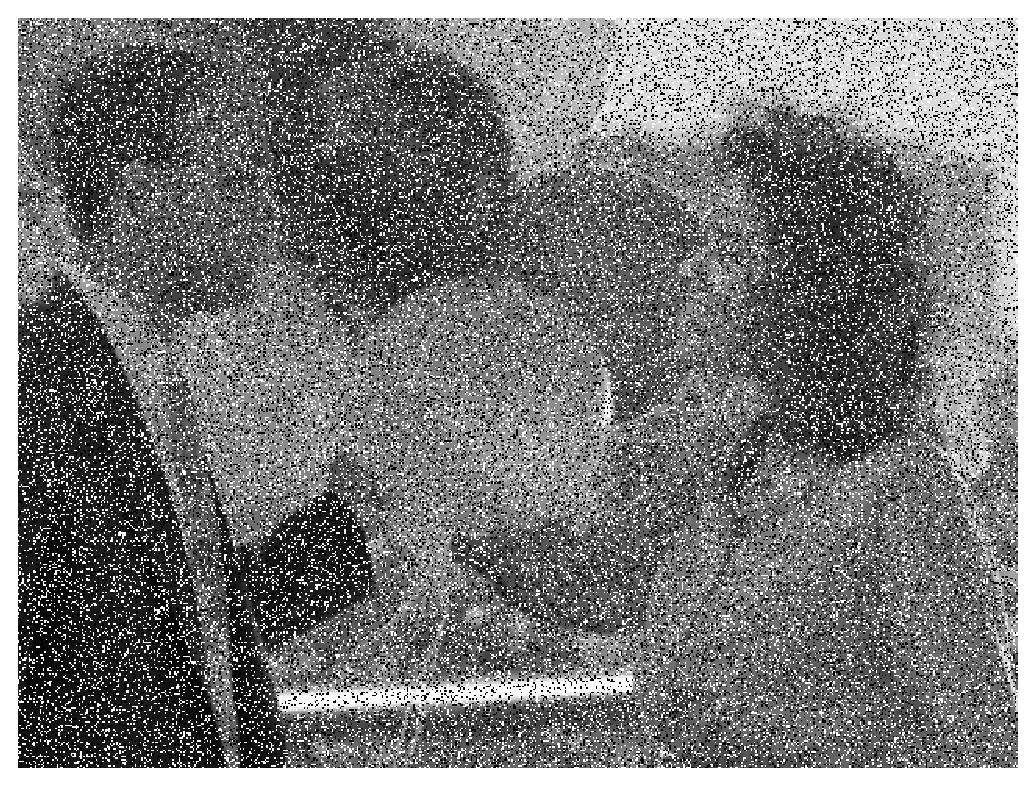
\includegraphics[height = 3cm, width = 3cm]{Figures/Prob5/Red/1}
					\caption{}
				\end{subfigure}
				\begin{subfigure}[h!]{.18\textwidth}
					\centering
					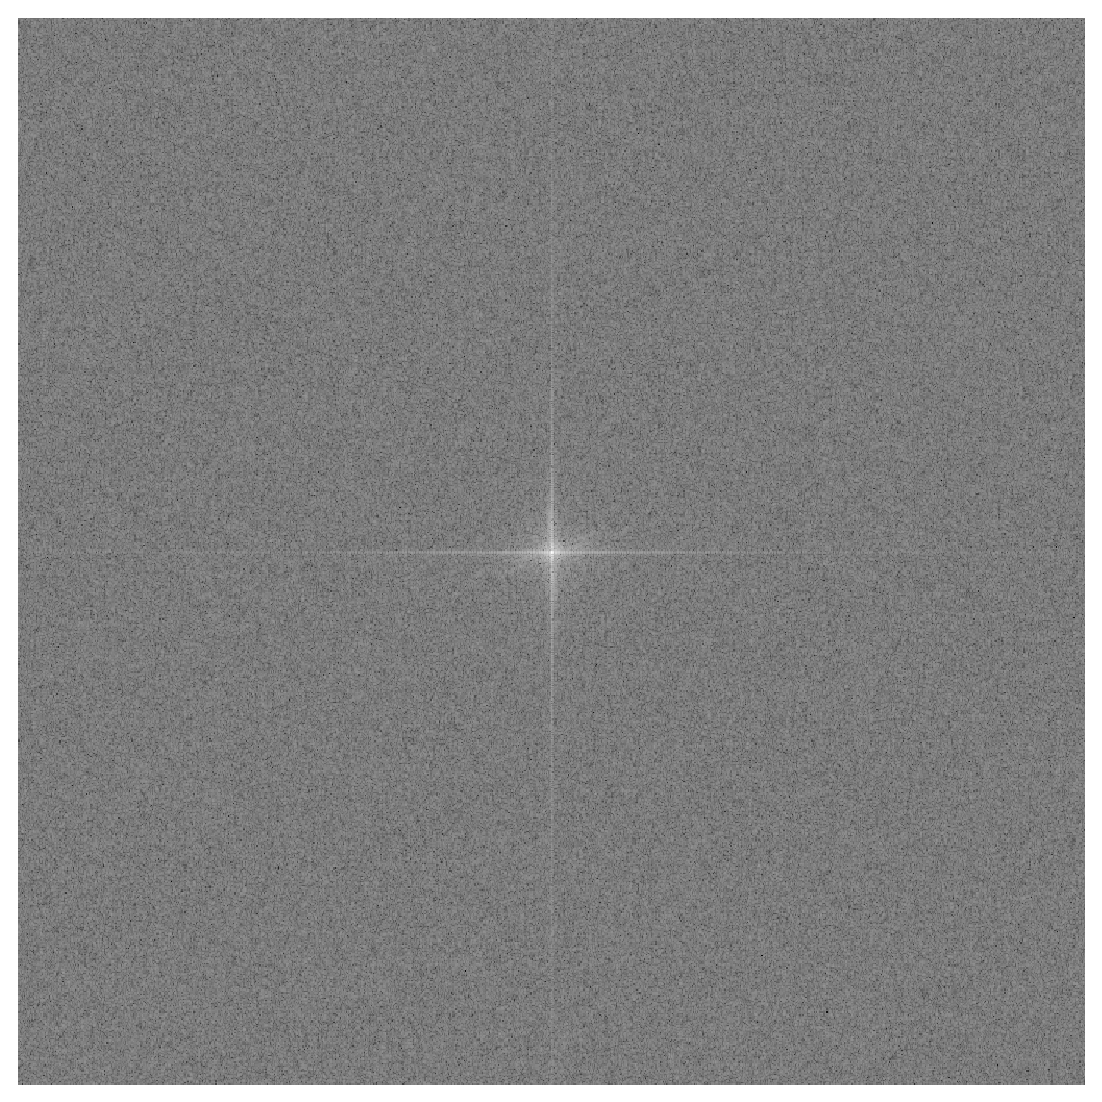
\includegraphics[height = 3cm, width = 3cm]{Figures/Prob5/Red/4}
					\caption{}
				\end{subfigure}
				\begin{subfigure}[h!]{.18\textwidth}
					\centering
					
\includegraphics[height = 3cm, width = 3cm]{Figures/Prob5/Red/5}
					\caption{}
				\end{subfigure}
				\begin{subfigure}[h!]{.18\textwidth}
					\centering
					\includegraphics[height = 3cm, width = 3cm]{Figures/Prob5/Red/6}
					\caption{}
				\end{subfigure}
				\begin{subfigure}[h!]{.18\textwidth}
					\centering
					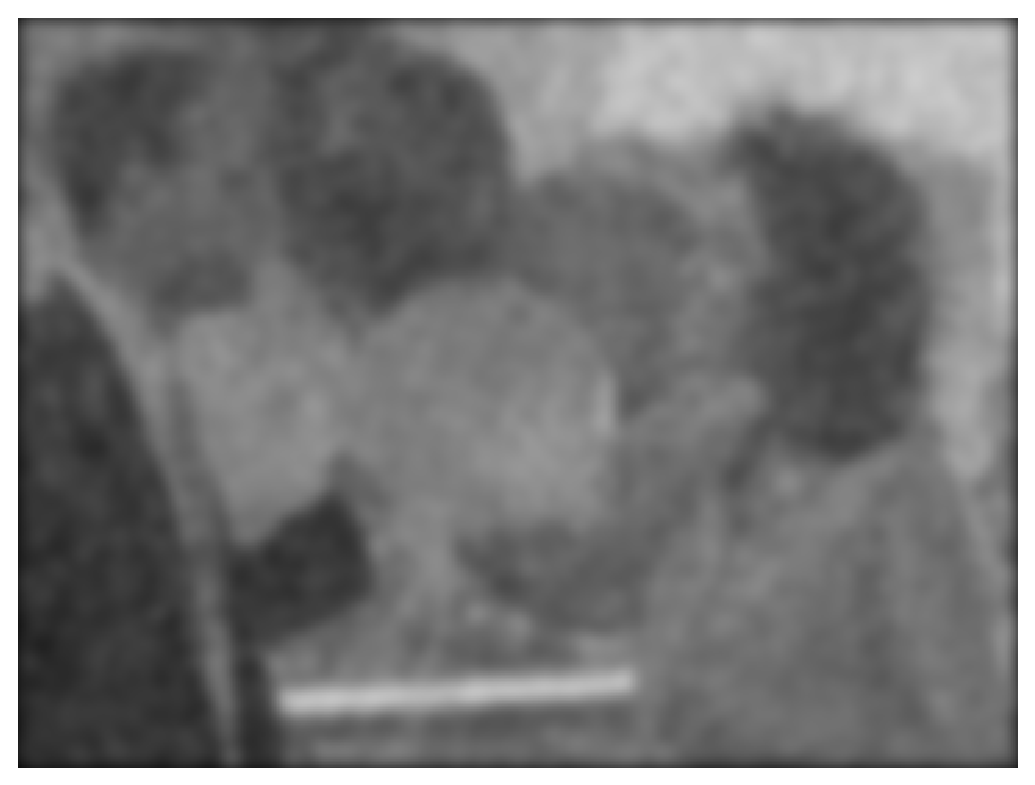
\includegraphics[height = 3cm, width = 3cm]{Figures/Prob5/Red/8}
					\caption{}
				\end{subfigure}
			\end{figure}
			\\ 
			\begin{figure}[h!]
				\centering
				\begin{subfigure}[h!]{.18\textwidth}
					\centering
					\includegraphics[height = 3cm, width = 3cm]{Figures/Prob5/Green/1}
					\caption{}
				\end{subfigure}
				\begin{subfigure}[h!]{.18\textwidth}
					\centering
					\includegraphics[height = 3cm, width = 3cm]{Figures/Prob5/Green/4}
					\caption{}
				\end{subfigure}
				\begin{subfigure}[h!]{.18\textwidth}
					\centering
					\includegraphics[height = 3cm, width = 3cm]{Figures/Prob5/Green/5}
					\caption{}
				\end{subfigure}
				\begin{subfigure}[h!]{.18\textwidth}
					\centering
					\includegraphics[height = 3cm, width = 3cm]{Figures/Prob5/Green/6}
					\caption{}
				\end{subfigure}
				\begin{subfigure}[h!]{.18\textwidth}
					\centering
					\includegraphics[height = 3cm, width = 3cm]{Figures/Prob5/Green/8}
					\caption{}
				\end{subfigure}
			\end{figure}
			\\ 
			\begin{figure}[h!]
				\centering
				\begin{subfigure}[h!]{.18\textwidth}
					\centering
					\includegraphics[height = 3cm, width = 3cm]{Figures/Prob5/Blue/1}
					\caption{}
				\end{subfigure}
				\begin{subfigure}[h!]{.18\textwidth}
					\centering
					\includegraphics[height = 3cm, width = 3cm]{Figures/Prob5/Blue/4}
					\caption{}
				\end{subfigure}
				\begin{subfigure}[h!]{.18\textwidth}
					\centering
					\includegraphics[height = 3cm, width = 3cm]{Figures/Prob5/Blue/5}
					\caption{}
				\end{subfigure}
				\begin{subfigure}[h!]{.18\textwidth}
					\centering
					\includegraphics[height = 3cm, width = 3cm]{Figures/Prob5/Blue/6}
					\caption{}
				\end{subfigure}
				\begin{subfigure}[h!]{.18\textwidth}
					\centering
					\includegraphics[height = 3cm, width = 3cm]{Figures/Prob5/Blue/8}
					\caption{}
				\end{subfigure}
			\end{figure}
			\newpage
			Now when we combine the red, green, blue $f_{flt}$, we get:
			\begin{figure}[h!]
				\centering
				\includegraphics[width = .5\textwidth]{Figures/Prob5/Filtered}
			\end{figure}
			\\ \\
			\item Discuss the reason for the choice (including filter parameters such as cutoff frequency, etc.) and effectiveness of your filter, and the possible challenges in reduction of the type of noise in the above image.
			\\ \\
			So I chose to use the Gaussian Low Pass Filter because of the Salt and Pepper noise is similar to Gaussian noise.  So I first chose an average sized $r_0 = 30$ to get a nice median between smoothness and the removal of noise.  To use the filer on a colored image, I first separated the colored image into its RGB components.  Then I applied the filter to each component.  After doing so, I end up with 3 filtered images, which will represent the RGB Components of the final filtered image.  Lastly, I simply put the 3 filtered images together to ge the final result.  I think the final result came out okay, as we can still see some noise, but it does retain a lot of the actual image without making it too smooth.  The challenge in reduction with this type of noise would be finding better parameter values to get a perfect balance between sharpness and noise reduction.  
		\end{enumerate}
	\end{problem}


\end{document}
